\documentclass[a4paper,UKenglish,cleveref,autoref,thm-restate]{lipics-v2021}

\usepackage{booktabs}
\bibliographystyle{plainurl}

\title{Database Theory in Action: The CALM Boundary in Content-Addressed Knowledge Stores}

\author{Behnam Sour}{Bone and Joint Reconstruction Research Center, Iran University of Medical Sciences, Tehran, Iran}{sourbehnam1374@gmail.com}{https://orcid.org/0009-0002-3176-1956}{}

\authorrunning{B.\ Sour}

\Copyright{Behnam Sour}

\ccsdesc[500]{Theory of computation~Database theory}
\ccsdesc[300]{Theory of computation~Logic and databases}
\ccsdesc[300]{Theory of computation~Distributed computing models}

\keywords{CALM theorem, monotonicity, content addressing, incremental view maintenance, semi-naive evaluation, Merkle DAG}

\relatedversion{Full version, with all proofs, the Lean development, and measurement scripts:}
\relatedversiondetails[cite={}]{Preprint}{https://arxiv.org/abs/XXXX.XXXXX}

\supplementdetails[subcategory={Reference implementation, property suite, Lean 4 proofs}]{Software}{https://github.com/sourbehnam1374-beep/growth-closures}

\nolinenumbers

\begin{document}

\maketitle

\begin{abstract}
Content-addressed stores in the Git/IPFS tradition name every part by a recursive hash of its content. When the parts are not files but \emph{derived knowledge} --- the least-fixpoint closure of typed rules over a growing seed of atoms --- the storage layer walks, mostly unknowingly, into database theory: closure growth is conservative exactly when the rules are monotone, incremental maintenance is semi-naive evaluation, and the practitioner's most natural request --- ``store only the \emph{maximal} bindings'' --- runs head-on into the CALM theorem. This note carries the boundary across: under payload-determined (oblivious) side conditions, no rule system can store exactly the subset-maximal bindings at every seed, and in a content-addressed store the cost of violating monotonicity is not abstract coordination but the retraction of named, referenced parts --- a trilemma between conservativity, history independence, and maximal parsimony whose identity axis CALM itself does not express. We show the witness live (a real dangling SHA-256 address), give the resolution architecture the boundary forces, and measure that it bites: on a natural-language corpus, one 268-atom descriptor cohort implies ${\sim}10^{80.7}$ admissible bindings under the complete semantics, against 637 under the quotient view. The entire closure algebra, including semi-naive frontier locality with monotonicity and finitarity \emph{derived} from the rule format, is kernel-checked in a self-contained constructive Lean~4 development shipped with the full version.
\end{abstract}

\section{A storage layer walks into database theory}

A content-addressed knowledge store keeps a universe of typed parts --- here a four-level tower $\mathsf{Atom} < \mathsf{Block} < \mathsf{Section} < \mathsf{Root}$ --- where the address of a part is a collision-resistant hash of its payload and the addresses of its children, Merkle-DAG style~\cite{Merkle87,Sanjuan20}. Atoms are ingested; everything above them is \emph{generated} by finitary rules ($\mathsf{bind}$: $m \ge 3$ atoms sharing a descriptor form a $\mathsf{Block}$ when an MDL-style code-length test passes; $\mathsf{lift}$, $\mathsf{frame}$, $\mathsf{close}$ assemble the upper levels). The state of the store over a seed $S$ is the least fixpoint $K(S)$ of the rule operator --- a Datalog$^{\exists}$-flavoured saturation in which content addressing acts as collision-resistant Skolemization, placing the system in the Skolem-chase regime~\cite{FaginKMP05,Marnette09}.

Four hypotheses govern everything: \textbf{H1} finitary rules, \textbf{H2} \emph{payload-determined} side conditions (a rule instance fires as a function of its premises' payloads only, never of the ambient set), \textbf{H3} stratified acyclic generation, \textbf{H4} injective content addressing. Under H1--H4 the growth theory is classical closure algebra the moment it is stated as such: growth is \emph{conservative} ($S \subseteq S' \Rightarrow K(S) \subseteq K(S')$, with old parts keeping their exact addresses, so growth is auditable as a Merkle address-set diff); \emph{incremental} ($K(S \cup D) = K(K(S) \cup D)$, computable frontier-locally --- semi-naive evaluation~\cite{BancilhonR86,Ullman89}, with no deletion and no rederivation, the machinery DRed exists to provide for non-monotone views~\cite{GuptaMS93} simply never needed); \emph{history-independent} (the canonical fingerprint depends only on the union of ingested batches); and \emph{continuous} over directed families, licensing streaming. That these are one-line corollaries of Knaster--Tarski is precisely the point of this note: the storage question \emph{is} a database-theory question, and the community that owns the boundary results should know where they are landing.

\section{CALM travels}

The boundary appears the moment a practitioner asks the obvious question. Cohorts of $n$ atoms sharing a descriptor generate $\sum_{m \ge 3}\binom{n}{m}$ admissible blocks --- every sufficiently large subset binds once the largest does. ``So store only the $\subseteq$-\emph{maximal} bindings.'' Maximality, however, is the textbook non-monotone operator: aggregates inside recursion demand lattice monotonicity precisely because ``maximal set'' breaks it~\cite{RossSagiv97}. The general form of the obstruction is the CALM theorem --- conjectured by Hellerstein~\cite{Hellerstein10}, proved by Ameloot, Neven and Van den Bussche via relational transducer networks~\cite{AmelootNV13}, surveyed in~\cite{HellersteinAlvaro20}: \emph{a problem has a consistent, coordination-free distributed implementation if and only if it is monotone}, where consistency is confluence over input orderings and the coordination-free computations are captured by \emph{oblivious} transducers, deciding without global knowledge.

The dictionary between the two settings is exact (\cref{tab:dict}); ``oblivious'' and ``payload-determined'' are the same condition wearing different clothes. Under it, the practitioner's request instantiates the only-if direction:

\begin{theorem}[localized form; full version Thm.~11, kernel-checked]
No payload-determined side condition yields, at every seed, exactly the $\subseteq$-maximal admissible bindings.
\end{theorem}

\begin{table}[t]
\caption{The correspondence. The last row is the axis the storage setting adds.}\label{tab:dict}
\centering\small
\begin{tabular}{ll}
\toprule
CALM / transducer networks & content-addressed closure \\
\midrule
consistency (confluence over orderings) & history independence of the fingerprint \\
oblivious transducer & payload-determined rule (H2) \\
monotone query & monotone one-step operator \\
non-monotone $\Rightarrow$ coordination & maximality $\Rightarrow$ global re-binding \\
--- (no notion of part identity) & conservativity: stages embed \emph{at identical addresses} \\
\bottomrule
\end{tabular}
\end{table}

The witness is four atoms and one delta, and it runs: at seed $S_3$, a three-atom binding $B_{123}$ is maximal and is stored at address \texttt{362db034e4f1\ldots}; one further atom arrives, the four-atom binding becomes the maximum, $B_{123}$ loses maximality, and under the ``maximal-only'' semantics its address --- referenced by a $\mathsf{Section}$ built at stage one --- now dangles. Nothing abstract happened: a named part was retracted. That is what the CALM boundary \emph{means} in a content-addressed store, and it is the element the classical formulation has no vocabulary for: CALM speaks of consistency and coordination, never of identity. Packaged as a trilemma: \textbf{(C)} conservativity as address-stable embedding, \textbf{(H)} history independence, \textbf{(P)} extensional maximal parsimony --- jointly unsatisfiable under H2, with (C)${\wedge}$(P) already contradictory. The contribution claimed is the formulation and its mechanization, not the boundary itself; the boundary is CALM's.

\section{What the boundary forces}

Three resolutions exhaust the trilemma's faces, and they are design patterns the systems world has been converging on ad hoc. The \emph{complete field} keeps every admissible binding --- (C)${\wedge}$(H), monotone, the closure itself. The \emph{subsumption-quotient view} stores the complete field but serializes only non-subsumed bindings --- (H)${\wedge}$(P) spent in the view, well-founded because subsumption follows strict kernel-set inclusion. \emph{Versioned cohort objects} make the maximal binding a mutable head over an immutable chain --- and this is the storage-layer analogue of the distribution-aware relaxations of CALM~\cite{ZinnGL12,AmelootKNZ15}: granting the system knowledge beyond individual payloads buys back behaviour that obliviousness forbids. One principle covers all three: \emph{keep identity and storage monotone and complete; spend parsimony in views}.

\section{Does it bite? One corpus, one number}

A reproducible stress proxy: atoms are the 8{,}631 sentences of \emph{Moby-Dick}; the descriptor of a sentence is its most frequent non-stopword token. The cohort distribution is heavy-tailed (\cref{fig:cohorts}): 3{,}078 descriptors, 637 bindable cohorts, maximal cohort $n = 268$ (\texttt{ahab}). Under the complete semantics the implied block count is ${\sim}10^{80.7}$ --- dominated by that single cohort, beyond physical storage; the quotient view materializes 637 blocks; cohort objects, 3{,}078 records. The resolutions are not optional optimizations --- on natural data the trilemma is operative. Crucially, \emph{complete identity survives}: every one of the $10^{80.7}$ bindings has a well-defined address computable on demand (H4 is a function, not a table), so the field stays canonical while only a linear-size representation is materialized. On the cost side, the frontier-local increment is measured at $6$--$10\times$ over batch reclosure for a fixed 20-atom delta on bases up to 8{,}000 atoms, with bit-identical fingerprints asserted throughout --- semi-naive evaluation, cashed out at the storage layer.

\begin{figure}[t]
\centering
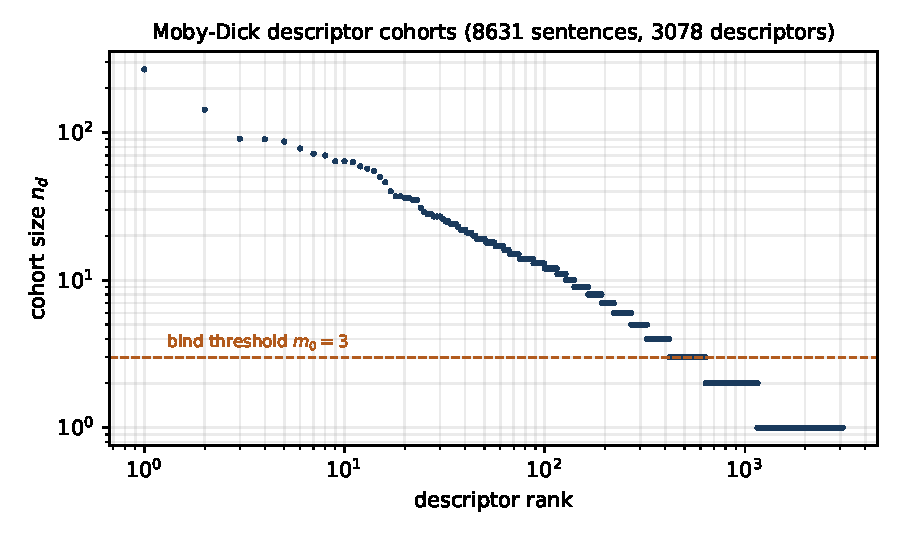
\includegraphics[width=0.62\linewidth]{fig_cohorts.pdf}
\caption{Descriptor-cohort sizes by rank (log--log) on \emph{Moby-Dick}. Everything above the dashed bind threshold ($m_0{=}3$) is bindable; the single 268-atom cohort drives the ${\sim}10^{80.7}$ complete-semantics blow-up.}\label{fig:cohorts}
\end{figure}

\section{Verified, and the question this exports}

Every theorem above --- the closure algebra, semi-naive frontier locality, and the impossibility witness (by \texttt{decide}) --- is kernel-checked in a self-contained, mathlib-free, fully constructive Lean~4 development; monotonicity and finitarity are \emph{derived} from the payload-determined rule format rather than assumed, both proofs axiom-free. The development, a pure-stdlib reference implementation with a 15-check SHA-256 ledger, a randomized property suite (${\sim}840$ adversarial instances), and the measurement scripts ship as ancillary files with the full version.

The connection runs both ways, and the return direction is the open problem this note hands to ICDT: \emph{principled deletion}. Content-addressed stores are grow-only by construction --- the trilemma above is exactly why --- yet redaction obligations are real. Which of conservativity, history independence, and frontier locality survive under tombstone (2P-set) semantics versus epoch re-closure, and at what identity cost, is a database-theory question that storage systems are currently answering ad hoc.

\bibliography{icdt_action_calm}

\end{document}
